\documentclass[12pt]{article}

\setlength{\oddsidemargin}{0in}  %left margin position, reference is one inch
\setlength{\textwidth}{6.5in}    %width of text=8.5-1in-1in for margin
\setlength{\topmargin}{-0.5in}    %reference is at 1.5in, -.5in gives a start of about 1in from top
\setlength{\textheight}{9in}     %length of text=11in-1in-1in (top and bot. marg.) 

\usepackage[square,super]{natbib}
\usepackage{graphicx}
\usepackage[dvipsnames]{xcolor}

\usepackage{multirow}
\usepackage{subcaption}
\usepackage{setspace}
\usepackage{xfrac}
\usepackage{hyperref}
\usepackage{upgreek}
\usepackage{lscape}
\usepackage{mhchem}
\usepackage{longtable}
\usepackage{rotating}
%\usepackage{fancyhdr}

\hypersetup{colorlinks=true,citecolor=black,linkcolor=blue, urlcolor=blue}

\usepackage{tikz}
%\usepackage[numbers,super,comma,sort&compress]{natbib}
%\usepackage[scaled=0.95]{helvet}
%\renewcommand{\familydefault}{\sfdefault}
\usepackage{amssymb}
\usepackage{amsmath}
\usepackage{placeins}
\usepackage[final]{pdfpages}

\newcommand*{\citen}[1]{%
  \begingroup
    \romannumeral-`\x % remove space at the beginning of \setcitestyle
    \setcitestyle{numbers}%
    \cite{#1}%
  \endgroup   
}

\setlength{\parskip}{0pt}


\definecolor{C0}{HTML}{1F77B4}
\definecolor{C1}{HTML}{FF7F0E}
\definecolor{C2}{HTML}{2CA02C}
\definecolor{C3}{HTML}{D62728}
\definecolor{C4}{HTML}{9467BD}
\definecolor{C5}{HTML}{8C564B}
\definecolor{C6}{HTML}{E377C2}
\definecolor{C7}{HTML}{7F7F7F}
\definecolor{C8}{HTML}{BCBD22}
\definecolor{C9}{HTML}{17BECF}


\newcommand{\tcn}[1]{{#1}}
\newcommand{\tcr}[1]{{#1}}
%\newcommand{\tcr}[1]{\textcolor{red}{#1}}

\newcommand{\beginsupplement}{%
        \setcounter{table}{0}
        \renewcommand{\thetable}{S\arabic{table}}%
        \setcounter{figure}{0}
        \renewcommand{\thefigure}{S\arabic{figure}}%
        \renewcommand{\thepage}{S\arabic{page}}%
     }

%\pagestyle{fancy}
%\fancyhf{}
%\cfoot{S\thepage}

\begin{document}

\title{Extrapolating DFT towards the complete basis set limit: Lessons from the PBE family of functionals}

\date{Supplementary Material}

\author{P.~Kraus\thanks{E-Mail: peter.kraus@curtin.edu.au}}

\maketitle


%%%END OF FOOTNOTES%%%

%%%MAIN TEXT%%%%

\beginsupplement

\section*{Table of contents}
\begin{enumerate}
	\item List of methods used with the diet100 variant of the GMTKN55 database \hfill p.~S2
	\item Figures of results for the subsets of the ASCDB database \hfill p.~S3
    \item Figures of results for all methods used with the diet100 subsets of the GMTKN55 database \hfill p.~S5
\end{enumerate}

Additional supplemental files and archives in computer-readable form are available on Zenodo, see DOI: \href{http://dx.doi.org/10.5281/zenodo.4783007}{10.5281/zenodo.4783007}. An executable version of this archive is available on \href{https://mybinder.org/v2/zenodo/10.5281/zenodo.4783007/?filepath=index.ipynb}{Binder}.

\clearpage
\begin{table}[tbh]
    \caption{List of methods used with the diet100 variant of the GMTKN55 database. References correspond to functionals and parametrizations of dispersion corrections. \vspace{0.5em}}
    \centering
    \begin{tabular}{l|l|l|l}
    \hline
    \textbf{Method name} & \textbf{DFA type} & \textbf{Disp. type} & \textbf{Reference} \\ \hline
    BLYP-D3(BJ)       & GGA         & D3(BJ)  & \citenum{Becke1988,Lee1988,Grimme2011} \\
    PBE-D3(BJ)        & GGA         & D3(BJ)  & \citenum{Perdew1996,Grimme2011} \\
    revPBE-D3(BJ)     & GGA         & D3(BJ)  & \citenum{Zhang1998,Perdew1996,Grimme2011} \\
    B97-D3(BJ)        & GGA         & D3(BJ)  & \citenum{Grimme2006,Grimme2011} \\ \hline
    SCAN-D3(BJ)       & mGGA        & D3(BJ)  & \citenum{Sun2015a,Brandenburg2016}\\
    M06L-D3        & mGGA        & D3(0)   & \citenum{Zhao2006,Goerigk2011} \\
    B97M-V          & mGGA        & VV10    & \citenum{Mardirossian2015} \\ 
    B97M-D3(BJ)    & mGGA         & D3(BJ)  & \citenum{Mardirossian2015,Najibi2018} \\ \hline
    B3LYP-D3(BJ)      & single hyb. & D3(BJ)  & \citenum{Becke1993,Stephens1994,Grimme2011} \\
    $\omega$B97X-V  & single hyb. & VV10    & \citenum{Mardirossian2014} \\
    M052X-D3       & single hyb. & D3(0)   & \citenum{Zhao2006a,Goerigk2011} \\
    dlDF+D10        & single hyb. & DAS2010 & \citenum{Pernal2009,Podeszwa2010} \\ \hline
    DSD-BLYP-D3(BJ)   & double hyb. & D3(BJ)  & \citenum{Kozuch2013} \\
    B2PLYP-D3(BJ)     & double hyb. & D3(BJ)  & \citenum{Grimme2006a,Goerigk2011} \\
    PWPB95-NL       & double hyb. & VV10    & \citenum{Goerigk2011a,Hujo2011,Yu2014} \\
    PBE0DH-D3(BJ)    & double hyb. & D3(BJ)  & \citenum{Bremond2011,Bousquet2015} \\
    \hline
    \end{tabular}
\end{table}

\clearpage
\begin{figure}[p]
    \centering
    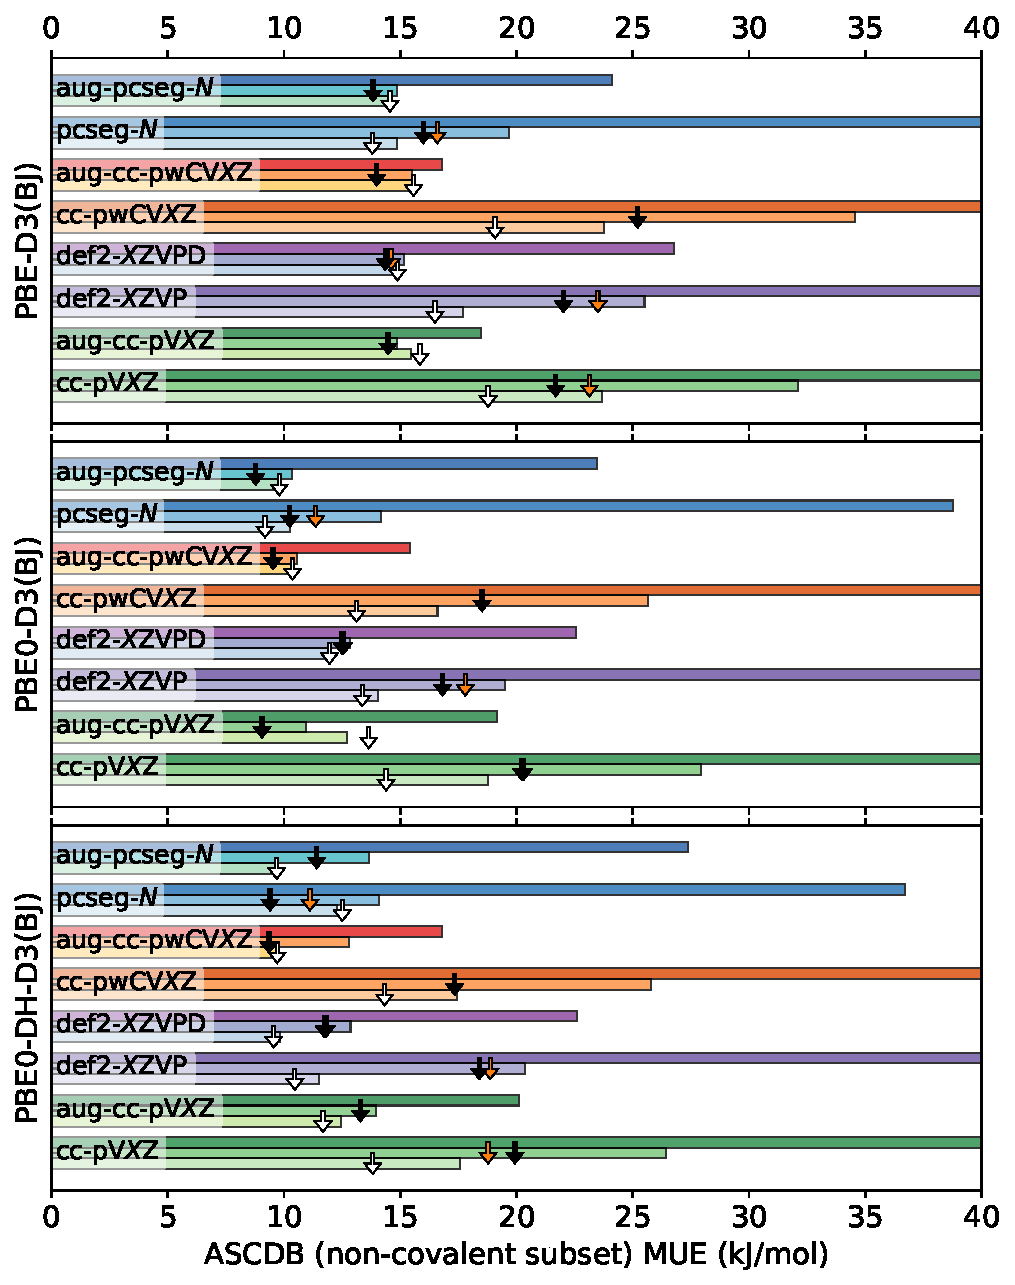
\includegraphics[width=8cm]{../output/fig_ascdb_nc.pdf}
    \caption{The total of the mean unsigned errors in the non-covalent subset of the ASCDB database. Calculations with 2-, 3-, and 4-$\zeta$ basis sets shown as bars. Results from the [2,3]-$\zeta$ extrapolation ($\bullet$) and [3,4]-$\zeta$ extrapolation ($\times$) from current work compared to previous [2,3]-$\zeta$ results (\textcolor{C1}{$\bullet$}), where available. \label{fig:ascdb-nc}}
    \vspace{1em}
    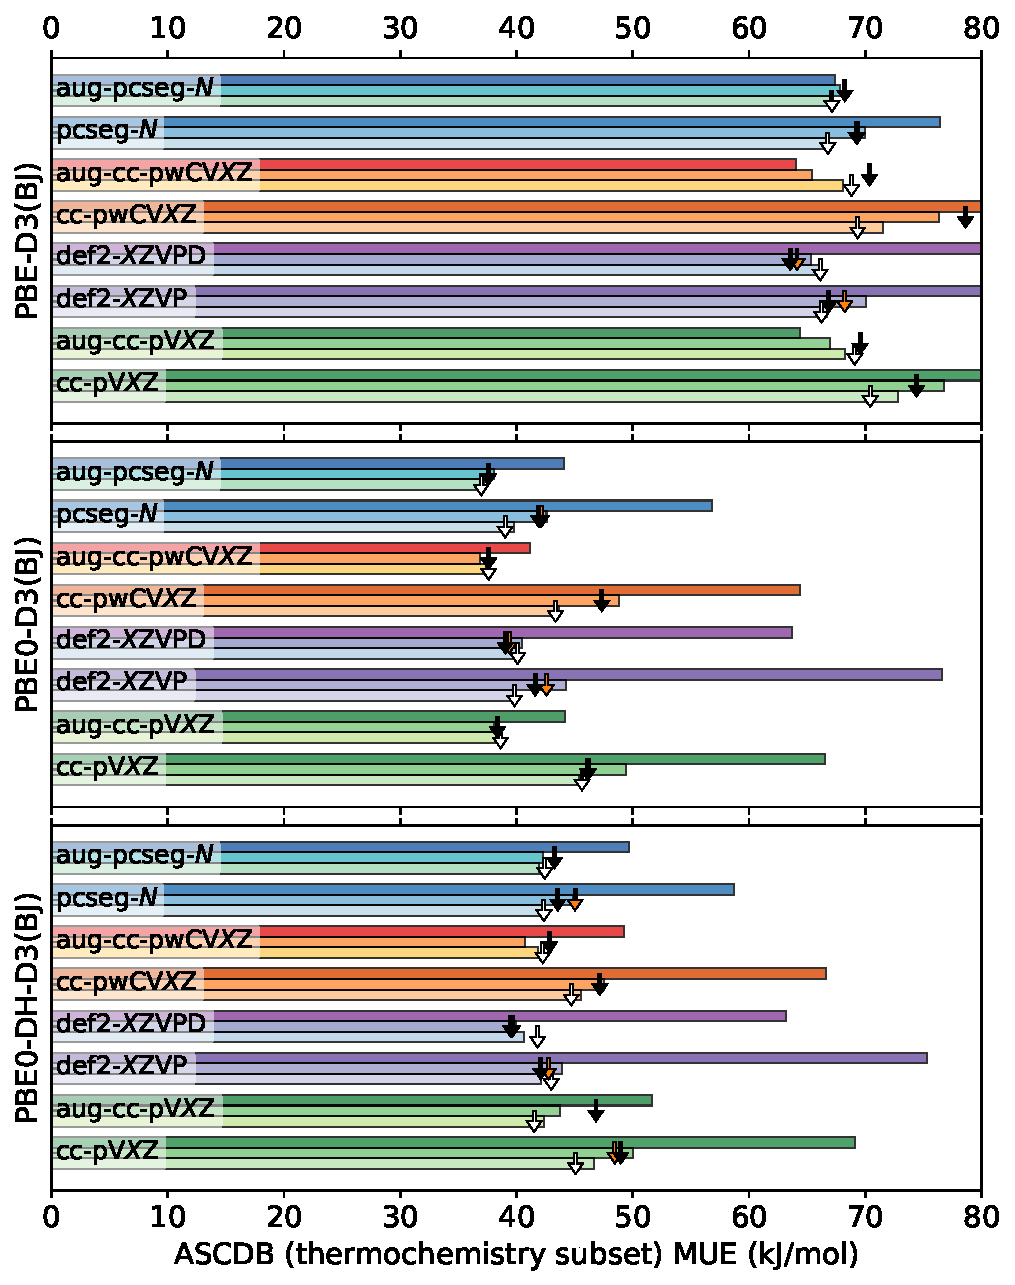
\includegraphics[width=8cm]{../output/fig_ascdb_th.pdf}
    \caption{The total of the mean unsigned errors in the thermochemistry subset of the ASCDB database. Bars and symbols as in Fig.~\ref{fig:ascdb-nc}.}
\end{figure}

\begin{figure}[p]
    \centering
    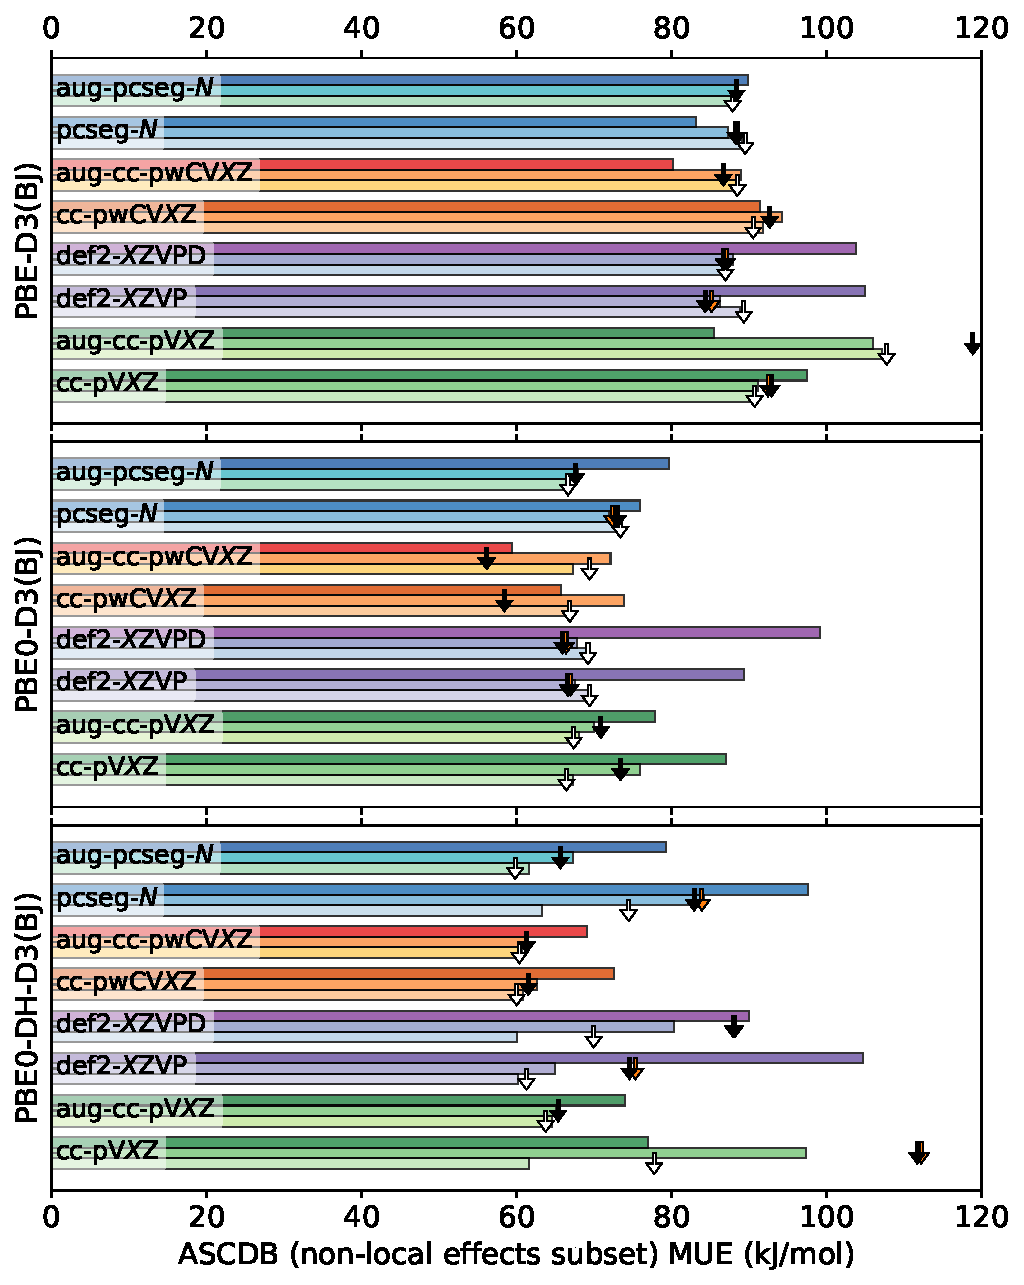
\includegraphics[width=8cm]{../output/fig_ascdb_nl.pdf}
    \caption{The total of the mean unsigned errors in the non-local subset of the ASCDB database. Bars and symbols as in Fig.~\ref{fig:ascdb-nc}.}
    \vspace{1em}
    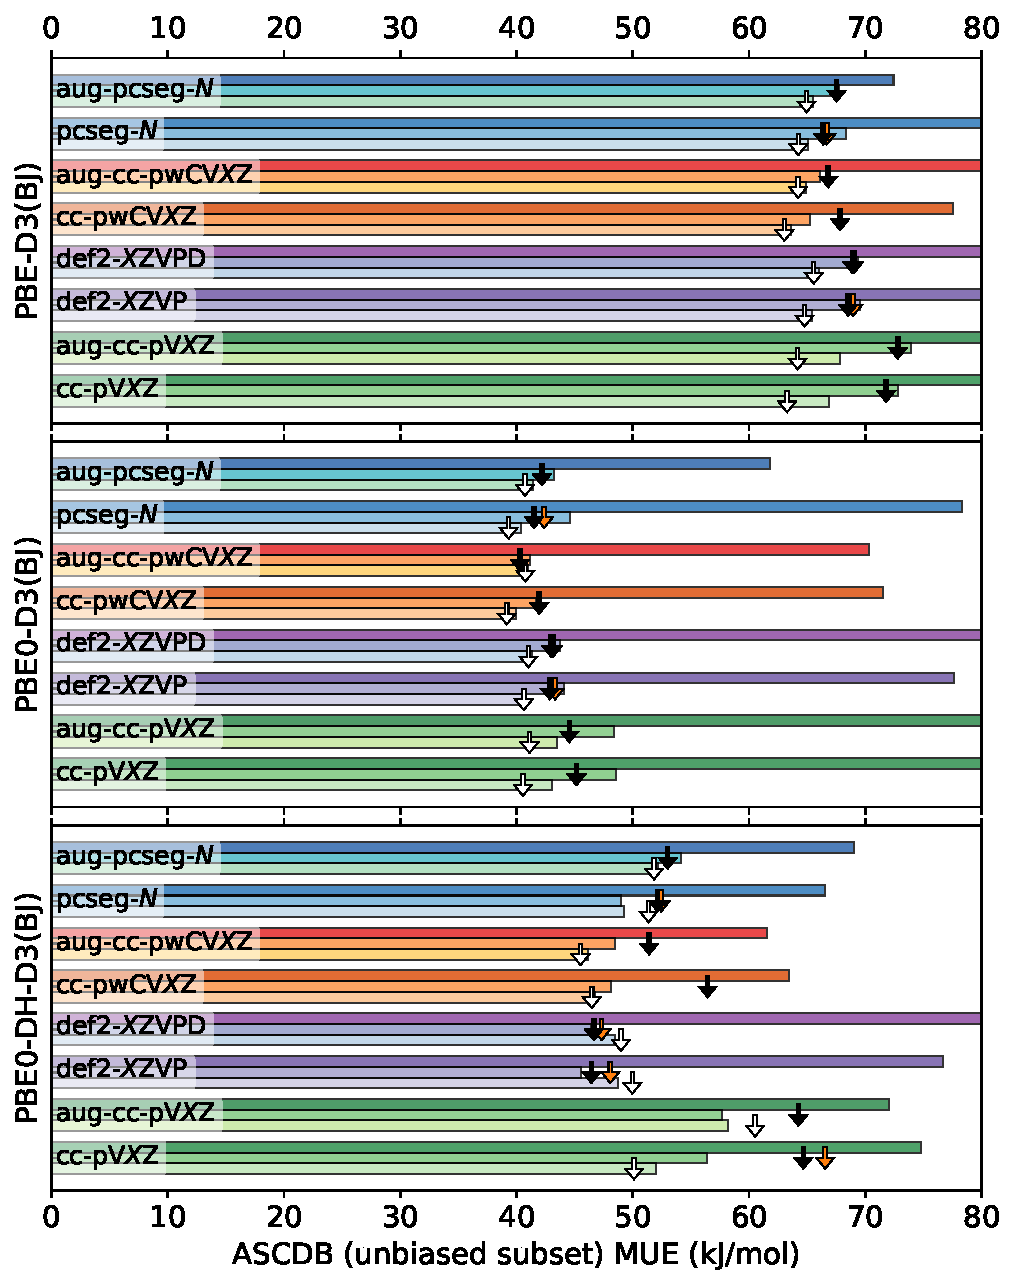
\includegraphics[width=8cm]{../output/fig_ascdb_ub.pdf}
    \caption{The total of the mean unsigned errors in the unbiased calculations subset of the ASCDB database. Bars and symbols as in Fig.~\ref{fig:ascdb-nc}.}
\end{figure}

\begin{figure}[p]
    \centering
    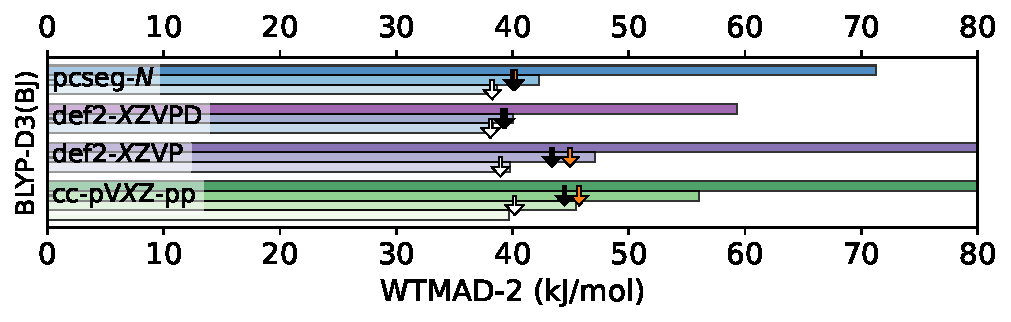
\includegraphics[width=8cm]{../output/fig_gmtkn55_00.pdf}
    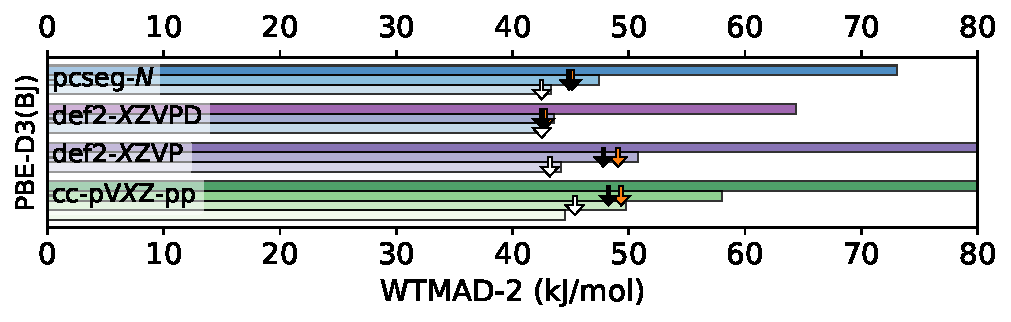
\includegraphics[width=8cm]{../output/fig_gmtkn55_01.pdf}
    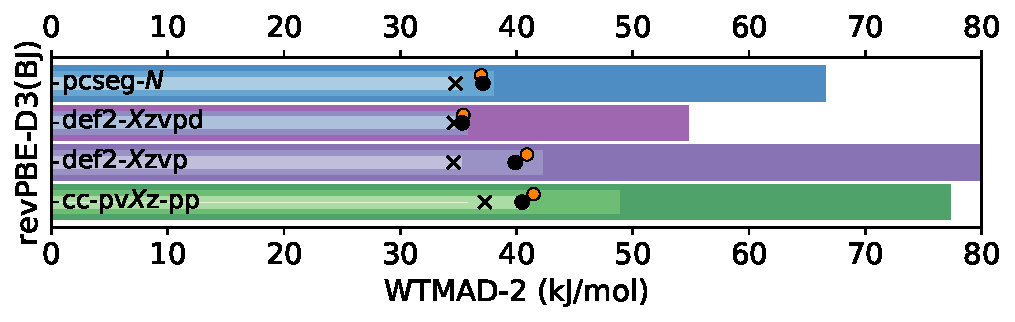
\includegraphics[width=8cm]{../output/fig_gmtkn55_02.pdf}
    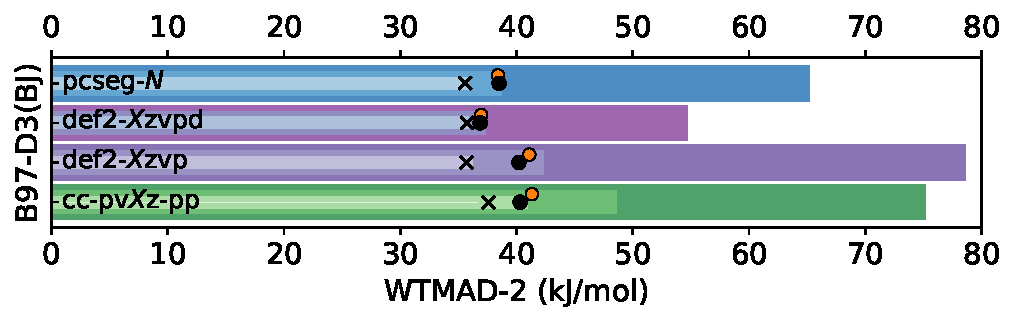
\includegraphics[width=8cm]{../output/fig_gmtkn55_03.pdf}
    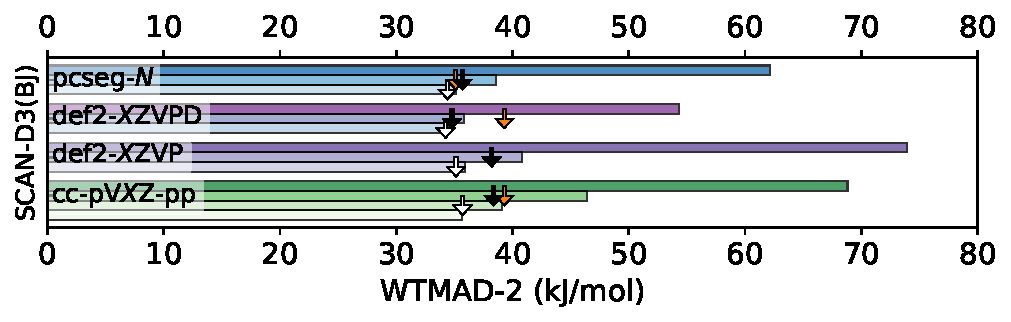
\includegraphics[width=8cm]{../output/fig_gmtkn55_04.pdf}
    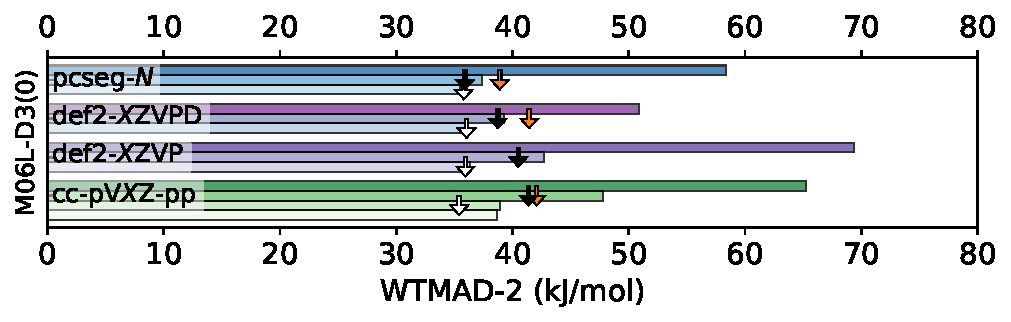
\includegraphics[width=8cm]{../output/fig_gmtkn55_05.pdf}
    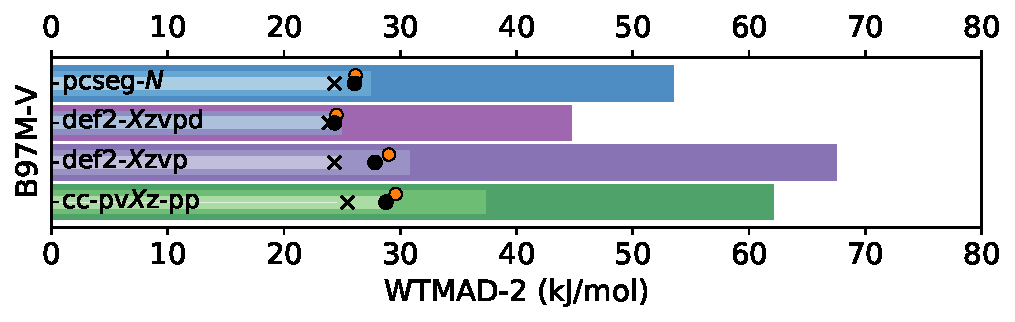
\includegraphics[width=8cm]{../output/fig_gmtkn55_06.pdf}
    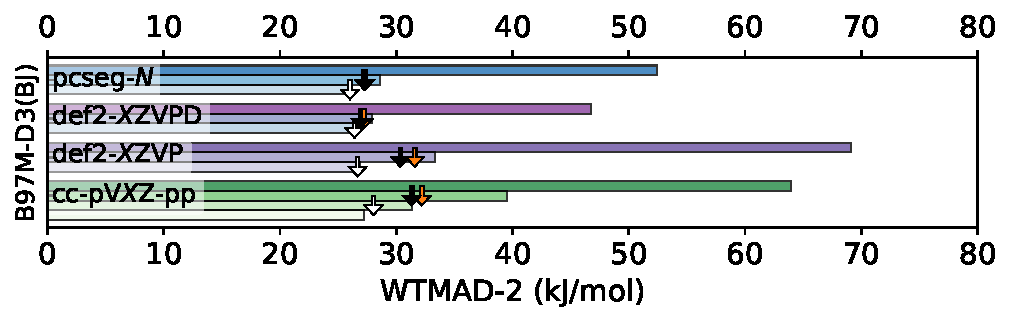
\includegraphics[width=8cm]{../output/fig_gmtkn55_07.pdf}
    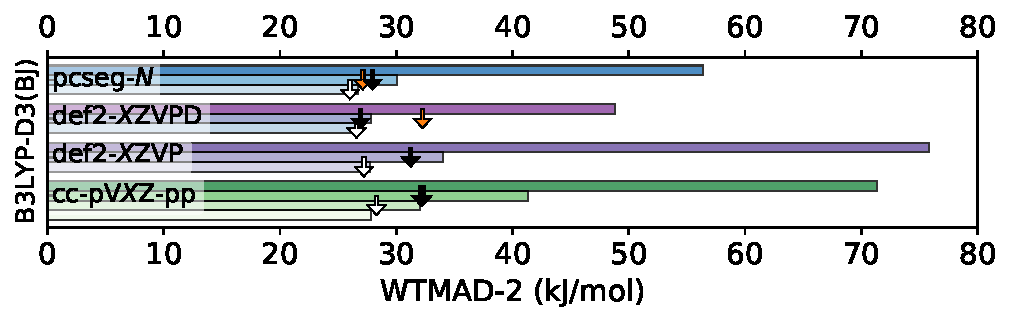
\includegraphics[width=8cm]{../output/fig_gmtkn55_08.pdf}
    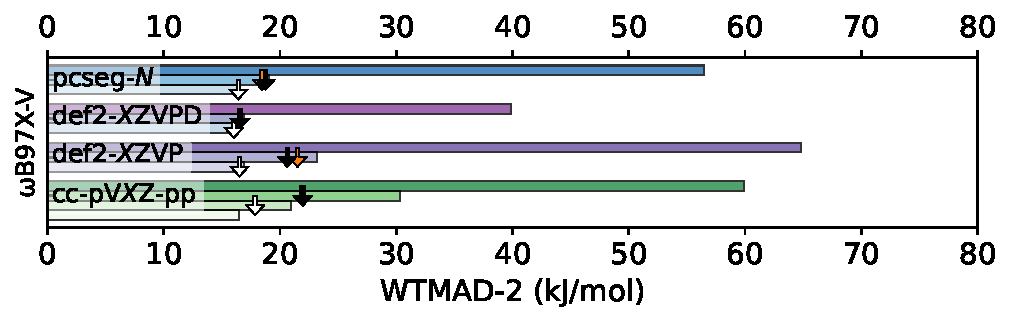
\includegraphics[width=8cm]{../output/fig_gmtkn55_09.pdf}
    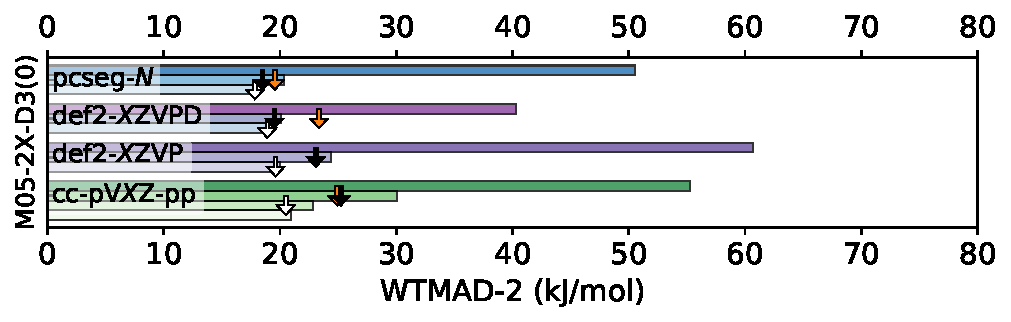
\includegraphics[width=8cm]{../output/fig_gmtkn55_10.pdf}
    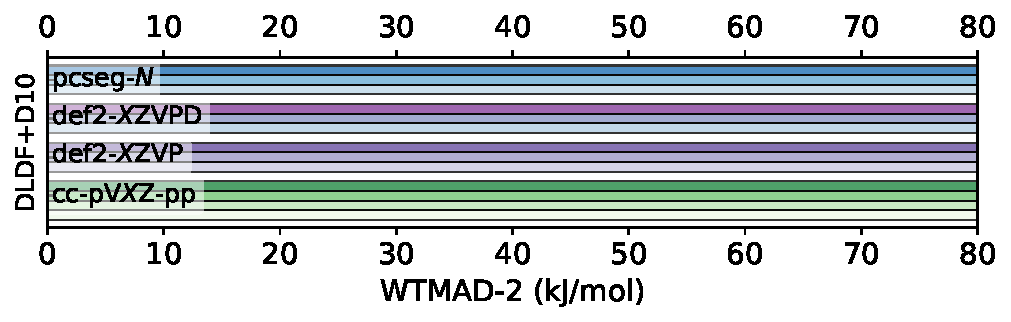
\includegraphics[width=8cm]{../output/fig_gmtkn55_11.pdf}
    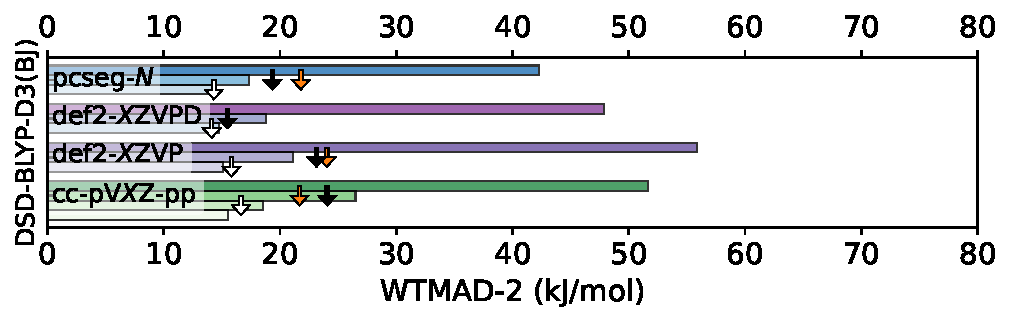
\includegraphics[width=8cm]{../output/fig_gmtkn55_12.pdf}
    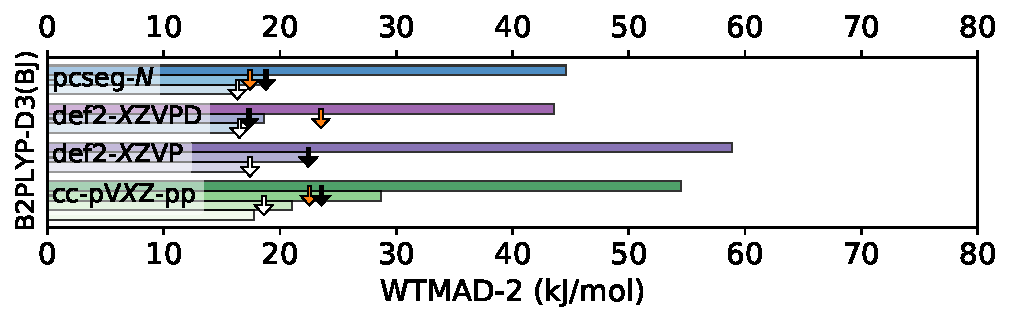
\includegraphics[width=8cm]{../output/fig_gmtkn55_13.pdf}
    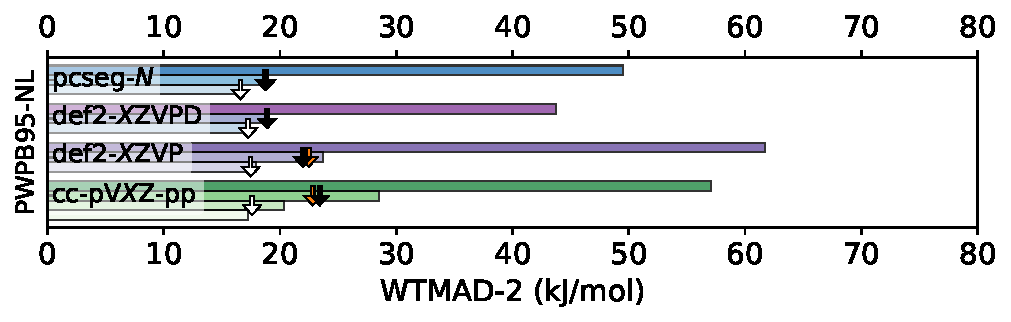
\includegraphics[width=8cm]{../output/fig_gmtkn55_14.pdf}
    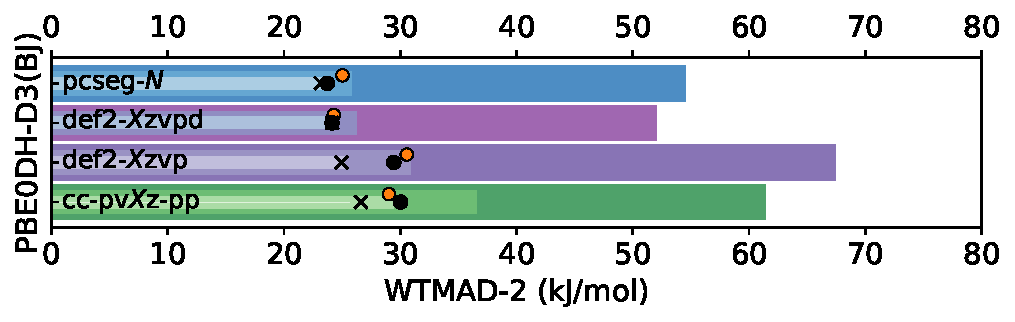
\includegraphics[width=8cm]{../output/fig_gmtkn55_15.pdf}
    \caption{The WTMAD-2 measures of the diet100 subset of the GMTKN55 database. Bars and symbols as in Fig.~\ref{fig:ascdb-nc}.}
\end{figure}

\clearpage
\bibliography{DFT_xtpl.bib}
\bibliographystyle{ieeetr}

\end{document}
